Este capitulo destina-se a apresenta��o dos dispositivos e programas, bem como os algoritmos, fun��es e metodologias utilizadas para projetar e implementar a FFT. Todos os passos apresentados aqui foram embasados na teoria apresentada no Capitulo (\ref{cap:RevisaoLiteratura}).

O desenvolvimento de um \text{hardware} para c�lculo de uma FFT em FPGA, abrindo m�o de IPs prontas e blocos de DSPs, utilizando apenas as bibliotecas padr�o de componentes, como a \textit{IEEE 1164} e a \textit{UNISIM}, disponibilizadas pelo fabricante, � uma tarefa que exige um projeto e implementa��o eficiente. Para o projeto da arquitetura  da FFT, � necess�rio ter conhecimento de toda a base matem�tica, tanto da Transformada de Fourier, quanto do algoritmo CORDIC e de suas variantes, para que se possa tirar o m�ximo proveito das simplifica��es e otimiza��es matem�ticas poss�veis. Na implementa��o do algoritmo, um design eficiente dos diferentes componentes que formam o \text{hardware}, al�m de reduzir a lat�ncia dos sinais, tamb�m reduz o consumo de Flip-Flops, LUTs, \textit{Muxes} e blocos de mem�ria. Tornando, assim,  poss�vel a implementa��o de uma \text{hardware} mais eficiente dentro das restri��es de recursos da FPGA.
	
Para que fosse poss�vel testar as funcionalidades e o desempenho ap�s a implementa��o, desde o inicio do projeto da FFT, fora elaborado o seguinte diagrama representativo:

\vspace{6mm}
\begin{figure}[H]
	\centering
	\captionsetup{width=0.9\textwidth, font=footnotesize, textfont=bf}	
	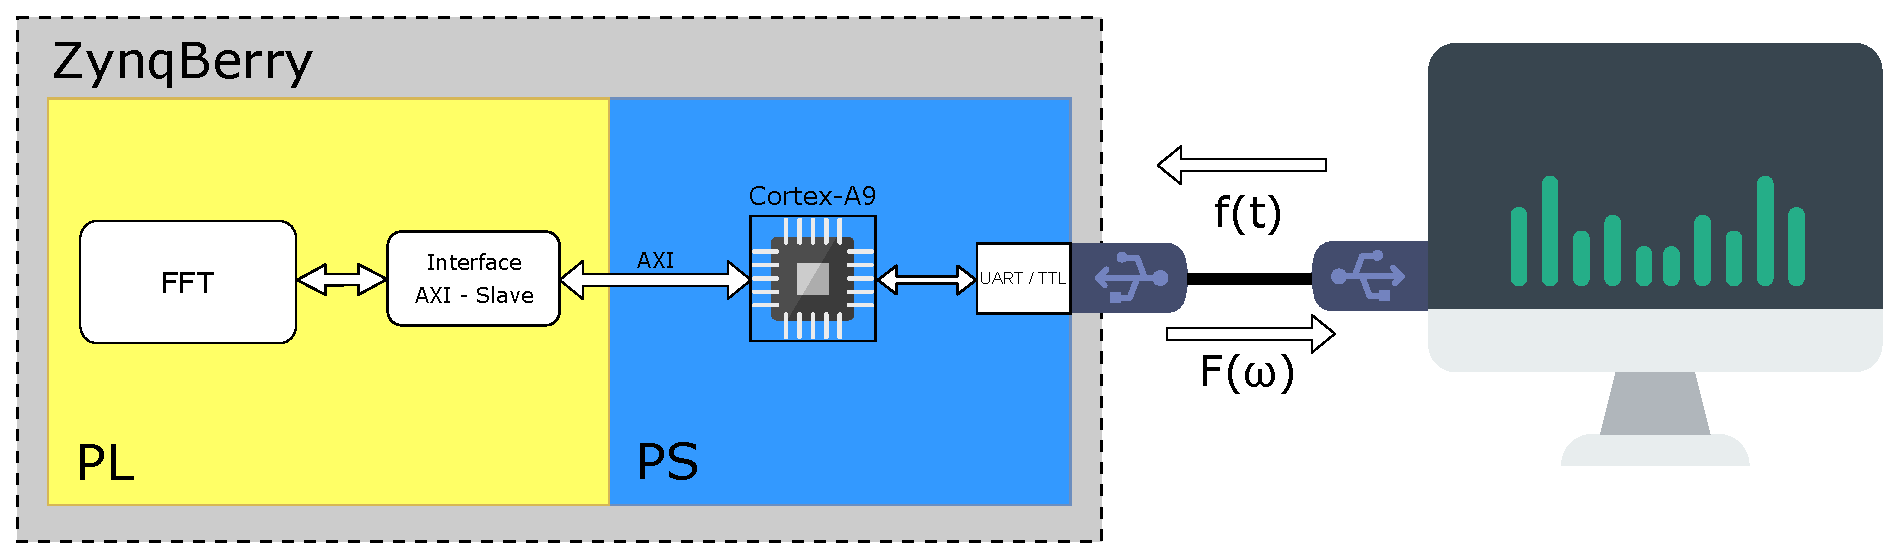
\includegraphics[width=0.9\linewidth]{Images/MateriaisMetodos/SistemaImplementacao.eps}
	\caption{Diagrama Geral do Sistema Implementado}
	\vspace{-3.5mm}
	\caption*{Fonte: Autoria Pr�pria}
	\label{fig:SistemaImplementacao}
\end{figure}
\vspace{6mm}

Como pode ser percebido na Figura (\ref{fig:SistemaImplementacao}), no sistema desenvolvido neste trabalho os dados de entrada da FFT, que pode ser dados amostrados ou simplesmente gerados por \textit{software}, s�o enviados por um computador via USB, pelo protocolo de comunica��o UART - TTL, para dentro da parte PS do placa ZynqBerry. Os dados s�o encaminhados pelo processador Cortex-A9 para o endere�o do \textit{hardware} de Interface AXI, o qual finalmente disponibiliza os dados de entrada ao m�dulo FFT implementado. Ap�s computado os dados de sa�da da FFT fazem o caminho reverso, para ent�o serem enviados ao computador via UART. Assim, este � o diagrama geral utilizado como guia, ao longo de todas as etapas do desenvolvimento, que est�o apresentados nas pr�ximas se��es.

\section{ZynqBerry TE0726-03M}
	O dispositivo escolhido para a implementa��o do algoritmo Radix-2 � o  \textit{ZynqBerry - TE0726} da fabricante \textit{Trenz Eletronic$^\circledR$}, apresentado na figura (\ref{fig:ZynqBerry-TE0726}). Este dispositivo � baseado no SoC (\textit{System On Chip}) Raspberry Pi modelo 2, vem equipado com uma FPGA SoM (\textit{System on Module}) XC7Z010-1CLG225C-REV3, da fam�lia Zynq-700 fabricada pela \textit{Xilinx$^\circledR$} \cite{trenz}. 

\vspace{6mm}
\begin{figure}[H]
	\centering
	\captionsetup{width=0.6\textwidth, font=footnotesize, textfont=bf}	
	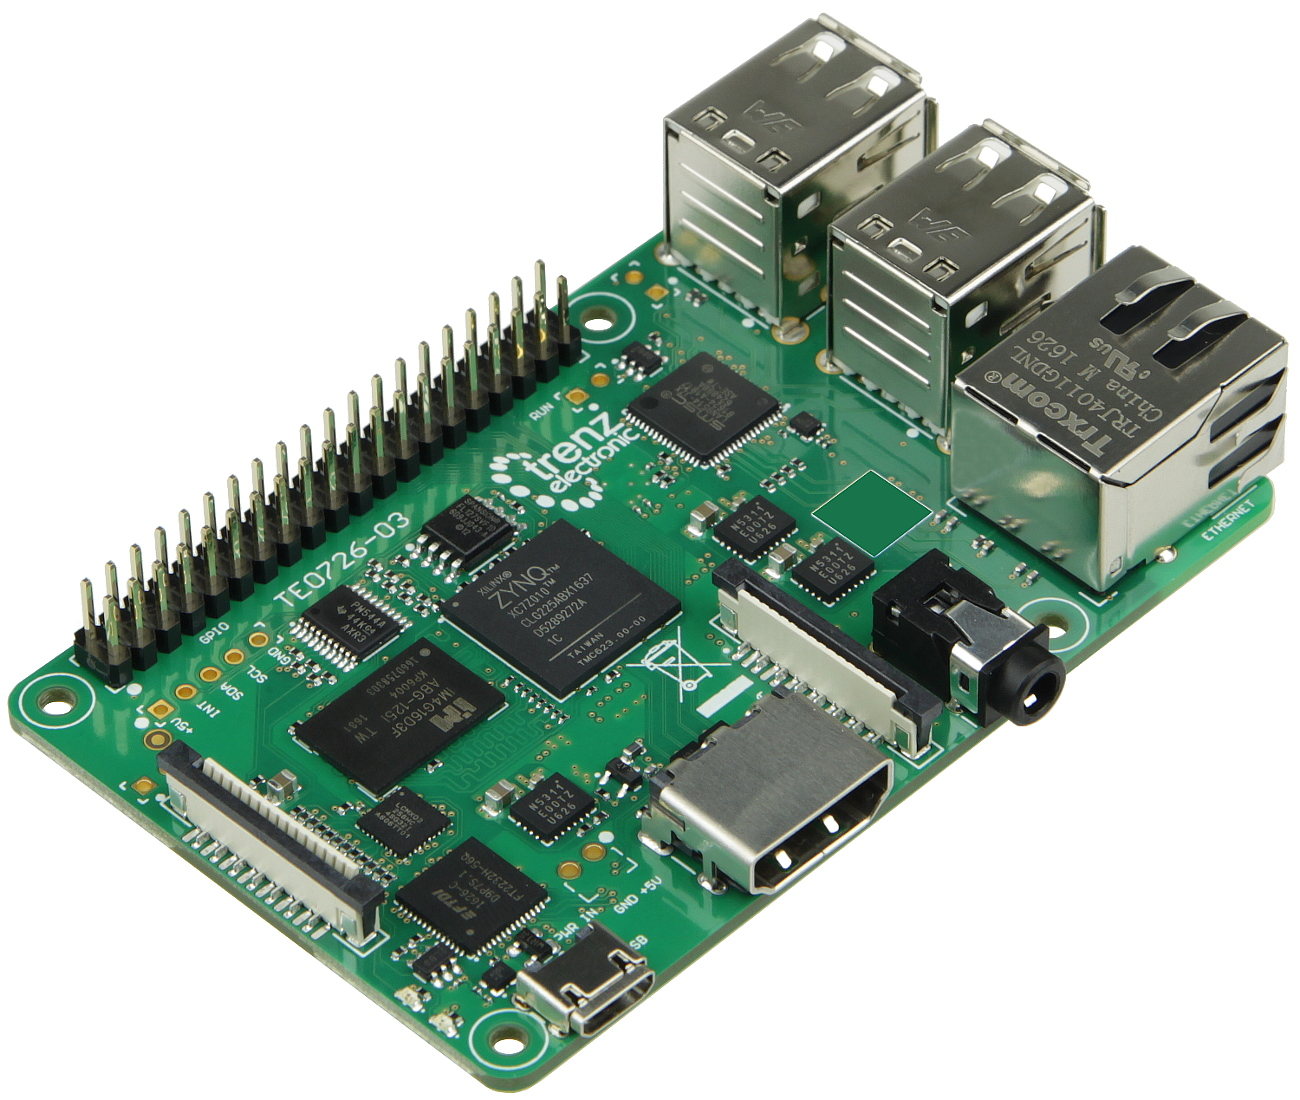
\includegraphics[width=0.6\linewidth]{Images/RevisaoDeLiteratura/TE0726-03M_0.jpg}
	\caption{SoC ZynqBery - TE0726}
	\vspace{-3.5mm}
	\caption*{Fonte: \citeonline{trenz}}
	\label{fig:ZynqBerry-TE0726}
\end{figure}
\vspace{6mm}


A FPGA XC7Z010-1CLG225C tem a mesma arquitetura dos modelos da fam�lia Artix-7, tamb�m da Xilinx, e contendo recursos como: 28.000 c�lulas l�gicas, 17.600 LUTs, 2.1 Mb de mem�ria RAM divididos em blocos de 26Kb e um total de 36.200 \textit{flip-flops}. Cada CLB, nesta FPGA, para implementar diferentes opera��es l�gicas utiliza 16 \textit{flip-flops}, 2 somadores de 4 \textit{bits} cascate�veis e ainda 8 LUTs, sendo poss�vel configurar a memoria RAM das LUTs para 64x1 ou 32x2 bits, ou ainda como um  \textit{shift register (SRL)}. Al�m disso, esta FPGA possuir 80 blocos DSP, cada um equipado com um multiplicador 18x25 simples, e um somador/acumulador de 48 bits. Todas estes recursos fazem do XC7Z010 um \textit{hardware} competente para as mais diversas aplica��es de processamento de sinais, como o calculo da FFT.

O processador utilizado no ZynqBerry TE0726-03M � um dual-core ARM Cortex-A9 de 866MHz, que proporciona um desempenho significativo em Sistemas Operacionais \sigla[Sistema Operacional]{S.O.},  como o sistemas baseados em kernel Linux, que podem incluem interface gr�fica sofistica. Cada n�cleo deste processador conta ainda uma unidade NEON\texttrademark  Media Processing Engine (MPE), para alto desempenho em codifica��o e decodifica��o de �udio e v�deo, e uma unidade de ponto flutuante para incremento da precis�o em opera��es matem�ticas.  Aliando a versatilidade da XC7Z010 e o poder de processamento do ARM Cortex-A9, � poss�vel construir um sistema que execute uma vers�o do S.O. Linux, tirando proveito de toda a funcionalidade de tal sistema operacional pode prover, e que ainda disponha de um \textit{hardware} acelerador personalizado para uma aplica��o especifica, e que trabalhe em paralelo a uma alta frequ�ncia. Provendo assim uma solu��o engenhosa de alto desempenho para processamento de sinais.

\section{Implementando Processador Cordic}
	Como apresentado na Se��o (\ref{section:Cordic}), devido a limita��es em disponibilidade de blocos multiplicadores nas FPGAs, se faz necess�rio ultilizar o algoritmo Cordic implementado em \textit{hardware} para realizar as opera��es de rotacionamento do vetor $H_r$ pelo �ngulo descrito por $W_{N_o}^r$. 

A FPGA XC7Z010-1CLG225 possui ao total 80 blocos de DSP (\textit{Digital signal processing}), onde cada um deles possui um \textit{hardware} multiplicador. Tais multiplicadores seriam suficientes para implementar a fun��o de rota��o de vetores necess�ria ao c�lculo da FFT. Por�m como tais blocos est�o em pequena quantidade e s�o essenciais para uma vasta gama de aplica��es. Como a FFT � um recurso que raramente � implementado isoladamente, sendo mais comum encontrar a FFT como apenas um dos elementos constituintes de um aplica��o bem maior, evitar o uso de DSP para reserva-los a outros sistemas � pertinente.    

Nesta etapa ser� realizado o projeto e implementa��o em FPGA do processador Cordic utilizado para montar o bloco da FFT. Tal processador seguira o funcionamento do algoritmo MSR Cordic apresentado na Se��o (\ref{section:MSR-CORDIC}).

\section{Projeto dos Par�metros Cordic}

Como apresentado na Se��o (\ref{section:MSR-CORDIC}), a determina��o dos par�metros Cordic $\mu_i$, $\mu_j$, $s_i$, $s_j$, $I$ e $J$ da Equa��o (\ref{eq:MSR}) � feita com base na minimiza��o do erro de aproxima��o $\upepsilon$, descrito pela Equa��o (\ref{eq:OtimizacaoMSR}).
Para encontrar o conjunto �timo de par�metros Cordic � poss�vel utilizar uma variedade de algoritmos determin�sticos, j� que este sistema se assemelha a problemas cl�ssicos de otimiza��o. 

Na Se��o (\ref{section:TBS}) fora apresentado o algoritmo de otimiza��o TBS, o qual se destinava a determina��o do conjunto de par�metros Cordic para o EEASR. O EEASR possu� um conjunto de �ngulos elementares menores do que o MSR, e a fun��o de otimiza��o n�o inclu�a a redu��o do do erro de ganho $K_c$ em rela��o a unidade, j� que a compensa��o deste ganho era realizada em uma etapa independente atrav�s de uma pseudo-rota��o. Por�m ao se adaptar a equa��o de minimiza��o do TBS para o caso do MSR, e incluir no conjunto de solu��o os �ngulos elementares do MSR.

Segue abaixo o pseudo-c�digo utilizado para obter o conjunto �timo de par�metros Cordic. O vetor $r_{\theta}$ representa o conjunto de todos �ngulos elementares, e $r_p$ presenta o conjuntos dos ganhos $K_n$, ambos oriundos das diferentes combina��es entre os par�metros Cordic.

 
\vspace{3mm}
	\lstset{style=VHDL}
	\begin{lstlisting}[mathescape]
		% Inicializa��o
		$\displaystyle \phi_{\theta}(1,k)~=~r_{\theta}(k)~para~todo~k,$
		$\displaystyle \phi_p(1,k)~=~r_p(k)~para~todo~k,$
		
		%Acumula��o
		$\displaystyle FOR~i=1~to~N-1$
			$\displaystyle FOR~k=1~to~Z(S_2)$
				$\displaystyle Encontra~k'~tal~que~:$
					$\displaystyle \upepsilon ~=~ min \sqrt{(\phi_{\theta}(i,k')+r_{\theta}(k)-\theta )^2 + (\phi_p(i,k^*)*r_p(k)-1 )^2} : 1 \leq k^* \leq Z(S_3) $
				$\phi_{\theta}(i+1,k)~=~\phi_{\theta}(i,k')+r_{\theta}(k)$
				$\phi_p(i+1,k^*)~=~\phi_p(i,k^*) * r_p(k)$
			$\displaystyle END$
		$\displaystyle END$
		
		%Determina��o do �timo Global
		$\displaystyle Encontra~k^*~tal~que~$
			$\displaystyle \upepsilon ~=~ min \sqrt{(\phi_{\theta}(N,k^*)-\theta )^2 + (\phi_p(N,k^*)-1 )^2} : 1 \leq k^* \leq Z(S_3) $
		$\displaystyle Result(N)~=~K^*$
		
		%Determina��o do Caminho Solu��o
		$\displaystyle FOR~i=N~to~2$
			$\displaystyle Encontra~k'~tal~que~$
				$\displaystyle \upepsilon ~=~ min \sqrt{(\phi_{\theta}(i-1,k')+r_{\theta}(k)-\theta )^2 + (\phi_p(i-1,k^*)*r_p(k)-1 )^2} : 1 \leq k^* \leq Z(S_3) $
			$\displaystyle k^*=k'$
			$\displaystyle Result(i-1)=k'$
		$\displaystyle END$
	
	\end{lstlisting}
	\label{code:PCTBSAlterado}
\vspace{3mm}

Uma aten��o especial � dada para o vetor de �ngulos elementares $r_{\theta}$. Este vetor � preenchido com o valor de �ngulos obtidos pelo conjunto de combina��es poss�veis dos par�metros Cordic do MSR, atrav�s da Equa��o (\ref{eq:S3}), o qual � reescrita como:

\begin{eqnarray}
	\alpha = \sum_{i=1}^{I} \mu_{i}2^{-s_i (n)} \\
	\beta = \sum_{j=1}^{J} \mu_{j}2^{-s_j (n)} \\
	r_{\theta} =  tan^{-1} \left(\frac{\beta}{\alpha}\right) \\ 
	:~\mu_{i},\mu_{j} \in \{-1,0,1\} \\
	s_i,s_j \in \{0,1, \dots, S\} 
	\label{eq:S32}
\end{eqnarray}

Atrav�s das diferentes combina��es de par�metros uma variedade de possibilidades de �ngulos preenchem o vetor  $r_{\theta}$. Por�m h� um problema com o c�lculo do arco tangente para combina��es onde o  $(\alpha<0, \beta<0)$ e $(\alpha>0, \beta<0)$, pois nestes casos as opera��es de rota��o deslocariam o vetor para o 4� e  3� quadrantes respectivamente, o que deveria resultar em valores de �ngulos maiores que $\pi/2$. Por�m o arco tangente considera apenas valores dentro do intervalo $(-\pi/2, \pi/2)$. Para corrigir tal efeito basta aplicar a seguinte condi��o:

\begin{eqnarray}
	Se~\alpha<0~e~\beta<0:~~r_{\theta} =  tan^{-1} \left(\frac{\alpha}{\beta}\right) -\frac{\pi}{2} \\ 
	Se~\alpha<0~e~\beta>0:~~r_{\theta} =  tan^{-1} \left(\frac{\alpha}{\beta}\right) +\frac{\pi}{2} \\ 
\end{eqnarray}  
 
Alguns par�metros do MSR s�o determinados de acordo com as limita��es de complexabilidade e disponibilidade de \textit{hardware}, como � o caso do n�mero de itera��es Cordic $N$, o n�mero de termos SPT $N_{SPT}$, e o n�mero m�ximo de deslocamentos de \textit{bit} $S$. Para alguns valores fora observado a recomenda��o usual na literatura, em \cite{Chih}, \cite{Kuo}, \cite{Park} e \cite{Kamal}. 

O n�mero de itera��o Cordic $N$ impacta diretamente no n�mero de ciclos de \textit{clock} necess�rio para realizar a opera��o, e tamb�m impacta no erro final $\upepsilon$. Como observado em \citeonline{Chih}, � admiss�vel tomar $N$ como 3, e ainda obter um bom SQNR. J� o $N_{SPT}$ impacta tamb�m no desempenho do erro $\upepsilon$, mas afeta ainda a complexabilidade do \textit{hardware}, j� que mais termos SPT significa mais operadores de deslocamento de \textit{bit}. Como a inten��o � montar uma FFT de bom desempenho, com o maior n�mero de pontos poss�vel, $N_{SPT}=3$ � admiss�vel baseado no que � visto em \citeonline{Chih}.

A escolha do n�mero m�ximo de deslocamento de \textit{bits} $S$ plica na utiliza��o de \textit{barrel shifters} maiores, e tamb�m no aumento do volume de mem�ria necess�ria para guardar os conjuntos de par�metros Cordic, para utilizar durante as opera��es de rota��o. Quanto maior for $S$ mais liberdade � dado ao conjunto de �ngulos elementares, e mais f�cil � encontrar conjuntos que reduzam $\upepsilon$ dentro das restri��es. 

A arquitetura da FFT implementada neste trabalho � pensada de modo que o fluxo de dados de entrada possam vir do Sistema de Processamento (PS), mas tamb�m possibilite a entrada de dados advinda de ADC (\textit{Analog-to-digital Conversor}) Flash de \textit{bits} bits. Portanto as palavras bin�rias utilizadas para representar os sinais precisam ter no m�nimo 12 \textit{bits}.  Para evitar a ocorr�ncia de \textit{overflow} em uma estrutura como a FFT de 1024 pontos, onde h� 10 n�veis, e apenas um ponto de soma a cada n�vel, e os ganhos s�o pr�ximos da unidade, se faz necess�rio utilizar 16 \textit{bits} para a representa��o de sinais.

Logo para determinar um valor para $S$, foi implementado o Algoritmo (\label{{code:PCTBSAlterado}}) com auxilio do \textit{software} $Matlab^\circledR$. Para cada valor de $S \in \{1...16\}$ fora criado conjunto de par�metros Cordic, fixando $I=1$ e $J=2$ (Modo Normal), para a partir destes par�metros realizar opera��es de rotacionamento de vetores nos moldes da Equa��o (\ref{eq:MSR}). A partir destas opera��es de rotacionamento fora obtido o SQNR para cada valor de $S$, afim de medir o impacto que este par�metro tem no desempenho do algoritmo. O resultado deste teste � expresso na Figura (\ref{fig:DeterminacaoS}).

\vspace{5mm}
\begin{figure}[H]
	\centering
	\captionsetup{width=0.9\textwidth, font=footnotesize, textfont=bf}	
	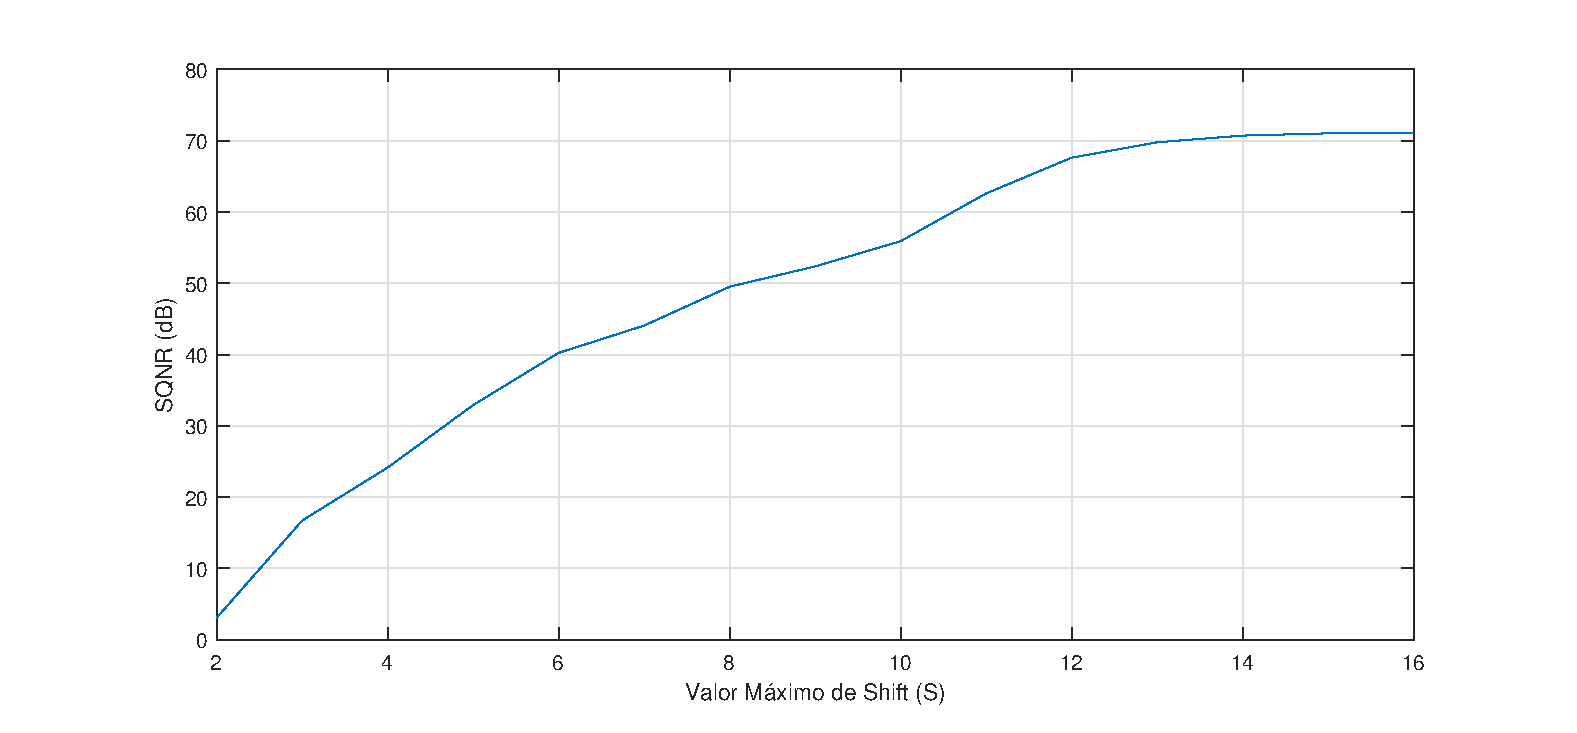
\includegraphics[width=0.9\linewidth]{Images/ImplementandoCordic/DeterminacaoS.eps}
	\caption{Rela��o entre $S$ e o SQNR M�dio para MSR Cordic Modo Normal}
	\vspace{-3.5mm}
	\caption*{Fonte: Autoria Pr�pria}
	\label{fig:DeterminacaoS}
\end{figure}    
\vspace{5mm}

Os conjuntos par�metros $s_i$ e $s_j$ para cada itera��o do algoritmo  ser�o armazenados em uma ROM de controle de cada Unidade Cordic. O n�mero de \textit{bits} necess�rios para armazenar estes par�metros � dado por $log(S)$. Como visto na Figura (\ref{fig:DeterminacaoS}) escolher $S=8$ promove um desempenho SQNR de $50dB$, e se faz necess�rio armazenar apenas $3$ \textit{bits} para cada elemento $s_i$ ou $s_j$. Por�m ao utilizar $4$ \textit{bits} para os mesmo fins � poss�vel fazer $S=16$, e alcan�ar um desempenho m�dio de $70dB$. Logo toma-se $S=16$ afim de alcan�ar o m�ximo desempenho poss�vel.

Com citado na Se��o (\ref{section:AnaliseDoErro}) os par�metros $I$ e $J$ podem ser constantes independente da opera��o de rota��o (Modo Normal), ou este podem variar a cada itera��o (Modo Generalizado). Com base no mesmo algoritmo implementado em $Matlab^\circledR$ apresentado anteriormente, foi inclu�do no vetor de �ngulos elementares $r$ as combina��es de par�metros poss�veis quanto tomado $N_{spt}=4$, para $(I=0,J=3)$,$(I=1,J=2)$, $(I=2,J=1)$ e $(I=3,J=0)$. E ent�o foram gerados os � conjuntos �timos de par�metros Cordic. 

O Modo Generalizado, para a simula��o proposta, apresentou um valor de SQNR de 92.9786 dB. O Modo Normal para o mesmo m�todo de simula��o apresentou um valor de 83.9786 dB. 

Segundo \cite{Chih}, para armazenar os par�metros $\{\mu_{i}, \mu_{j}\} \in \{-1,0, 1\}$, $\{s_i,s_j\} \in \{0,1,..,6\}$ de uma �nica intera��o do Algoritmo MSR Cordic, s�o necess�rios $(log(S)+2)N_{SPT}$ \textit{bits} para o modo Normalizado e $(log(S)+3)N_{SPT}$ para o Modo Generalizado. Ou seja o impacto do inser��o dos \textit{switches}, necess�rios no caso do Modo Generalizado, em termos de implementa��o � apenas a inclus�o de mais um \text{bit} no conjunto de dados de cada intera��o. Justificando portanto a escolha da implementa��o do MSR Cordic no Modo Generalizado.

Assim os dados referente aos par�metros escolhidos com base no Algoritmo (\ref{code:PCTBSAlterado}), para o MSR Cordic Modo Generalizado, com $N_{SPT}=3$ e $S=16$, s�o armazenados na forma bin�rio em uma componente ROM em VHDL. Esta ROM � presente e individual a cada unidade Cordic. 

\section{Arquitetura Cordic Implementada}
Ap�s a defini��o dos par�metros CORDIC, � ent�o realizada a implementa��o da arquitetura em FPGA, atrav�s da linguagem VHDL. Segundo \citeonline{Chih}, as opera��es de multiplica��o dos termos SPT em (\ref{eq:MSR}) podem ser realizadas utilizando operadores l�gicos de deslocamento de \textit{bit}, ou  \textit{shifters}. Como observado em (\ref{eq:MSR}), as duas partes $x$ e $y$ do sinal de entrada precisam ser deslocados para direita de forma diferenciada, com base nos par�metros $I$ e $J$, gerando assim cada parte $N_{SPT}$ sinais deslocados. 

As opera��es de deslocamento de $x$ e $y$ podem ser realizadas utilizando apenas dois \textit{Barrel shifters}, ambos com uma entrada e tr�s sa�das. O \textit{Barrel shifter} � um componentes l�gico capaz de deslocar um palavras bin�ria por um n�mero especifico de \textit{bits} utilizando apenas l�gica combinacional, o que possibilita efetuar a opera��o de deslocamento em apenas um ciclo de \textit{clock}. A �nica desvantagem deste componente � o n�mero elevado de multiplexadores necess�rios para sua implementa��o: $n log_2 n$, onde $n$ � o tamanho da palavra bin�ria. Por�m, como neste projeto $n=16$ \textit{bits}, admitiu-se o custo de inclus�o de 64 multiplexadores em prol de se obter o melhor desempenho na opera��o base do algoritmo CORDIC. 

Para a implementa��o em VHDL fora utilizado o diagrama de intera��o sugerido por \citeonline{Chih}, o qual segue na Figura (\ref{fig:ArquiteturaCordicGeneralizado}).

\vspace{5mm}
\begin{figure}[H]
	\centering
	\captionsetup{width=0.8\textwidth, font=footnotesize, textfont=bf}	
	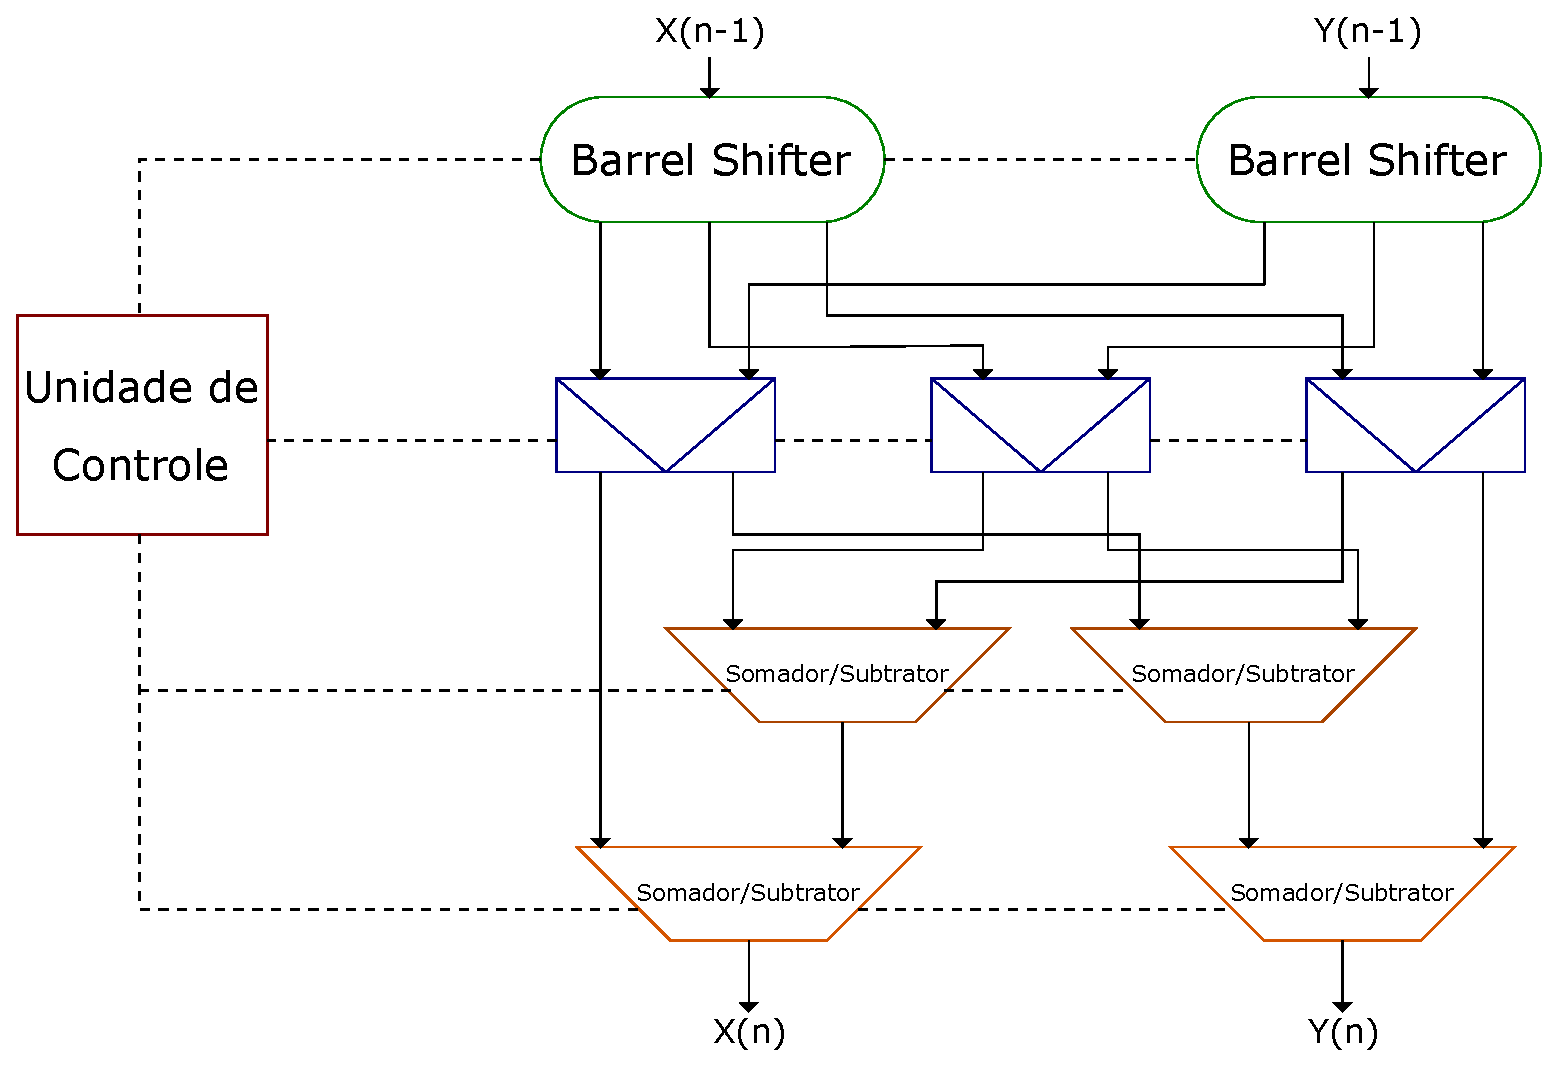
\includegraphics[width=0.8\linewidth]{Images/MateriaisMetodos/ArquiteturaCordicGeneralizado.eps}
	\caption{Arquitetura da Itera��o MSR Cordic Modo Normal $N_{spt}=3$}
	\vspace{-3.5mm}
	\caption*{Fonte: Adaptado \cite{Chih}}
	\label{fig:ArquiteturaCordicGeneralizado}
\end{figure}    
\vspace{5mm}

\vspace{5mm}
\begin{figure}[H]
	\centering
	\captionsetup{width=0.3\textwidth, font=footnotesize, textfont=bf}	
	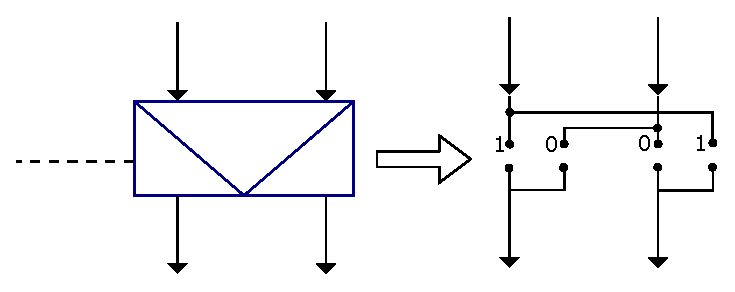
\includegraphics[width=0.3\linewidth]{Images/MateriaisMetodos/Sswitch.eps}
	\caption{Arquitetura Switch 2x2}
	\vspace{-3.5mm}
	\caption*{Fonte: Adaptado \cite{Chih}}
	\label{fig:Sswitch}
\end{figure}    
\vspace{5mm}

Como pode ser visto na Figura (\ref{fig:ArquiteturaCordicGeneralizado}), a implementa��o da intera��o CORDIC � feita basicamente de um conjunto de 4 somadores e 2 \textit{Barrel Shifters}. A implementa��o do Algoritmo CORDIC pode ser feita na forma sequencial ou na forma \textit{pipeline}. Na forma sequencial, a Unidade de Controle da Figura (\ref{fig:ArquiteturaCordicGeneralizado}), por meio de um conjunto de \textit{flip-flops}, armazenam o valor final da intera��o e retro alimentam a entrada do circuito, durante os $N$ ciclos de intera��o CORDIC. A cada intera��o a Unidade de Controle muda os par�metros de acordo com os dados presentes na ROM. Na forma de \textit{piperline} v�rias unidades CORDIC, como as vista Figura (\ref{fig:ArquiteturaCordicGeneralizado}), s�o encadeadas sequencialmente de modo que cada unidade seja respons�vel por uma intera��o separadamente, o que possibilita  a opera��o ser realizada em apenas um ciclo de \text{clock}.

Na forma sequencial a implementa��o do Algoritmo ocupa menos recursos da FPGA, j� que s�o necess�rios apenas um hardware de intera��o, e \textit{flip-flops} de controle. Apesar disso, o n�mero de ciclos de \textit{clock} necess�rios para concluir a opera��o � ditada pelas opera��es sequenciais do Unidade de Controle, que nunca ser� inferior a $N$ ciclos. Na forma \textit{pipeline}, o n�mero de ciclos de \textit{clock} necess�rios para finalizar a opera��o de rota��o  � dependente apenas da velocidade de propaga��o dos sinais, atrav�s do \textit{hardware} encadeado das itera��o. No entanto, como neste modo existem $N$ \textit{hardwares} de intera��o encadeados, o consumo de recursos da FPGA � bem maior. Por quest�o de limita��o de recursos da FPGA utilizada, se optou pela implementa��o na forma sequencial. 



 



\section{Implementando a FFT 16 Pontos}
	\label{sec:ImplementandoFFT16}
Ap�s implementado o processador CORDIC, � necess�rio montar uma primeira vers�o da FFT, para que seja poss�vel testar o desempenho do processador, e o consumo de recursos da arquitetura implementada. Ent�o, � escolhido montar uma FFT de apenas 16 pontos, o que demanda o uso de 8 unidades CORDIC, que ser�o suficientes para executar as 8 opera��es de rotacionamento vetorial por n�vel. A Figura (\ref{fig:ArquiteturaFFT16P}) apresenta o diagrama da arquitetura implementada.


\begin{figure}[H]
	\centering
	\captionsetup{width=1\textwidth, font=footnotesize, textfont=bf}	
	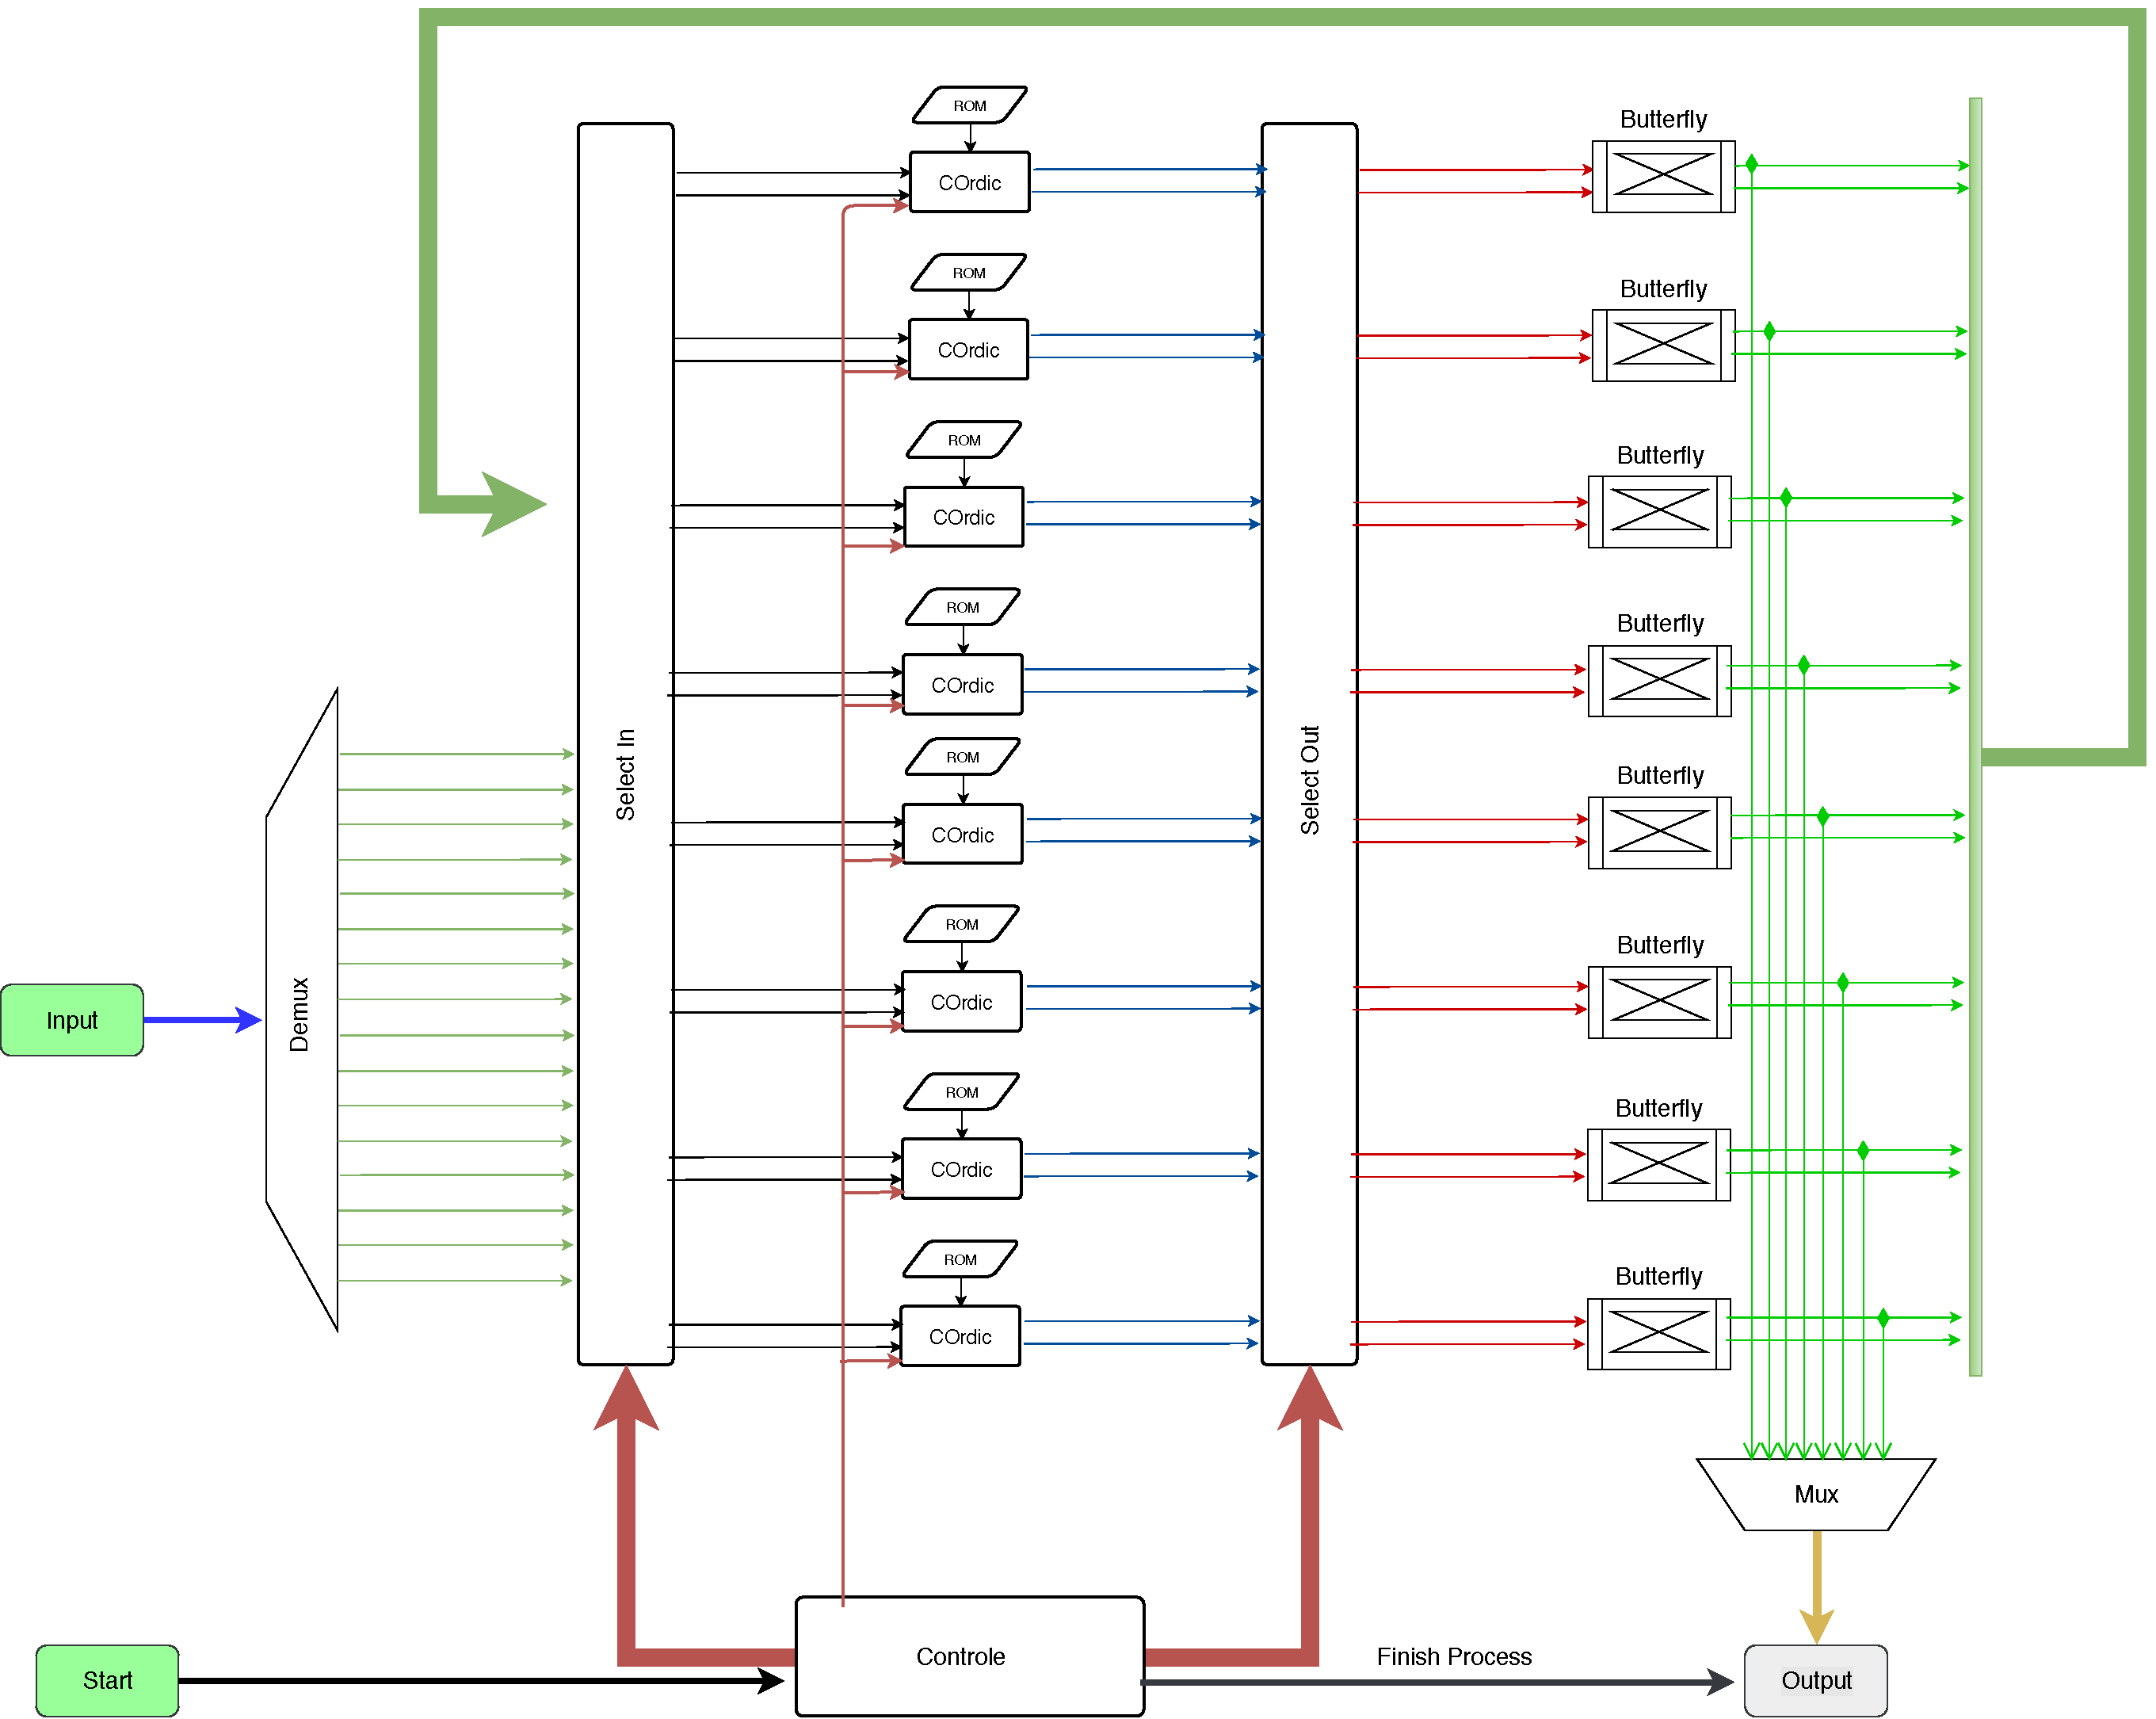
\includegraphics[width=1\linewidth]{Images/MateriaisMetodos/ArquiteturaFFT.pdf}
	\caption{Arquitetura Implementada FFT de 16 Pontos}
	\vspace{-3.5mm}
	\caption*{Fonte: Autoria Pr�pria}
	\label{fig:ArquiteturaFFT16P}
\end{figure}

Como visto na Figura (\ref{fig:ArquiteturaFFT16P}), para receber os dados de entrada serializados,  o \textit{Input} da FFT possui um \text{Demux}, assim como a porta \textit(Output) possui um \textit{Mux}, para devolver os dados computados. Para transferir tais dados seriais via AXI, o qual realiza a ponte entre o PS e o PL, � necess�rio implementar tal interface para testar a FFT.  A implementa��o do m�dulo AXI, utilizado como interface para as implementa��es de \textit{hardware} deste trabalho, podem ser vistas no Anexo (\ref{cap:AXI}). 

Ainda na Figura (\ref{fig:ArquiteturaFFT16P}), cada unidade CORDIC possui uma ROM, que armazena os conjuntos de par�metros otimizantes, os quais foram previamente calculados por (\ref{code:PCTBSAlterado}). A unidade \textit{Select Out} � respons�vel por ordenar, a cada itera��o, as sa�das das unidades CORDIC para o ordem adequada de entrada das unidades \textit{Butterfly}, de acordo com o diagrama da FFT por decima��o na frequ�ncia, apresentado em (\ref{fig:FFT8PDIF}). A unidade \textit{Select In}, na Figura (\ref{fig:ArquiteturaFFT16P}), realiza a sele��o da entrada de sinais nas unidades CORDIC, escolhendo entre o canal do \textit{Demux} dos dados de entrada, e o \textit{Feedback} da sa�da das unidades \textit{Butterfly}.

A arquitetura da Figura (\ref{fig:ArquiteturaFFT16P})  foi concebida de forma que a unidade \textit{Controle}, ap�s o recebimento do sinal de \textit{Start}, acione as unidades \textit{COrdic}, iniciando a opera��o de rota��o de vetores. Ap�s 3 ciclos de \textit{Clock}, os sinais de sa�da s�o direcionados pelo \textit{Select Out}, controlado pela Unidade \textit{Controle}, para as unidades \textit{Butterfly} que retroalimentam o bloco \textit{Select In}. Este processo que dura 3 ciclos de \textit{clock}, caracteriza o c�lculo de um n�vel da FFT. Como uma FFT de 16 pontos possui 4 n�veis, a unidade de Controle realiza 4 itera��es, retroalimentando as unidades \textit{COrdic} por meio do \textit{Select In}.

Ao final do processo de itera��o dos 4 n�veis da FFT, a unidade de Controle aciona o sinal de \textit{Finish Process}, sinalizando a Interface AXI que os dados j� foram computados, e j� podem ser transferidos ao PS de forma serial. Um ponto importante aqui, � que se faz necess�rio transferir apenas  metade dos sinais computados, pois o espectro de Fourier calculado � sim�trico. Logo, s�o transferidos os 8 primeiros pontos da FFT, obedecendo a ordem \textit{Bit-Reverse}, e compensando o m�dulo dos sinais, transferindo os 15 \textit{bits} mais significativos de cada ponto. 
	


\section{Implementando a Interface AXI}
	\label{cap:AXI}
Como citado na Se��o (\ref{sec:Zynq-7000}), na fam�lia de SoC Zynq-7000, o AXI � o meio padr�o pelo qual diferentes componentes dentro do ambiente PL se conectam, e mais importante, � o meio pelo qual componentes em PL se comunicam com o processador em PS. Como a implementa��o da FFT, realizada na Se��o (\ref{sec:ImplementandoFFT16}), � feita em PL, e se deseja enviar e receber dados da FFT via UART, ao computador fora da placa ZynqBerry, � preciso incluir uma Interface AXI.

Uma Interface AXI para este projeto deve ser capaz de converter os sinais de sa�da da FFT para um formato padronizado de comunica��o AXI. Segundo \citeonline{zynq-7000}, existem 3 tipos b�sicos de interfaces AXI: 

\begin{itemize}
	
	\item \textbf{AXI-Standard:} Interface destinada a transfer�ncias de dados em alta velocidade e de maior volume. Utiliza endere�amento de  mem�ria para acessar dados, e portanto consome recursos de mem�ria para ser implementado. Interface mais complexa, e oferece maiores op��es de controle de dados, inclusive transfer�ncia no modo \textit{brust}.
	
	\item \textbf{AXI-Lite:}Interface destinada a transfer�ncias de dados em baixa velocidade, e de menor volume.  Consome espa�o de mem�ria apenas para controlar dados da transfer�ncia, como destino, origem e status da transmiss�o. Interface mais simples do que a AXI-Standard, n�o oferece controle de dados como o modo \textit{brust}.
	
	\item \textbf{AXI-Stream:} Interface para transfer�ncia de dados em alta velocidade, por�m n�o utiliza mapeamento de mem�ria. Toda a transfer�ncia nesta interface � peita por em  fluxo de dados cont�nuos, os quais n�o s�o armazenados pela interface. 
	
\end{itemize} 

Teoricamente qualquer uma das 3 op��es de interface AXI seriam capazes de transmitir e receber os dados da FFT. Por�m deve ter em mente que uma interface AXI tamb�m consome recursos da FPGA, os quais devem ser destinados principalmente a FFT. Logo uma interface como a AXI-Standard n�o seria adequado, j� que n�o h� necessidade de utilizar recursos como controle de dados. Neste projeto � de interesse ter acesso seletivo aos dados de sa�da da FFT, de modo que seja poss�vel ao PS acessar os valores de amplitude de frequ�ncias especificas. Como a interface AXI-Stream n�o possui mapeamento de mem�ria, n�o seria de interesse utilizar esta interface. Portanto, ser� utilizada a interface  AXI-Lite.

O fabricante do Zynq-7010 que equipa a placa ZynqBerry, utilizada neste trabalho, disponibiliza em sua IDE de desenvolvimento, o Vivado HLx 2017.4, uma ferramenta de cria��o de IPs. Utilizando esta ferramenta, partindo design em VHDL da FFT, foi criado um novo perif�rico AXI, como pode ser visto nas Figuras (\ref{fig:FerramentaIPA}), (\ref{fig:FerramentaIPB}), (\ref{fig:FerramentaIPC}) e (\ref{fig:FerramentaIPD}).

\vspace{5mm}
\begin{figure}[H]
	\centering
	\captionsetup{width=0.8\textwidth, font=footnotesize, textfont=bf}	
	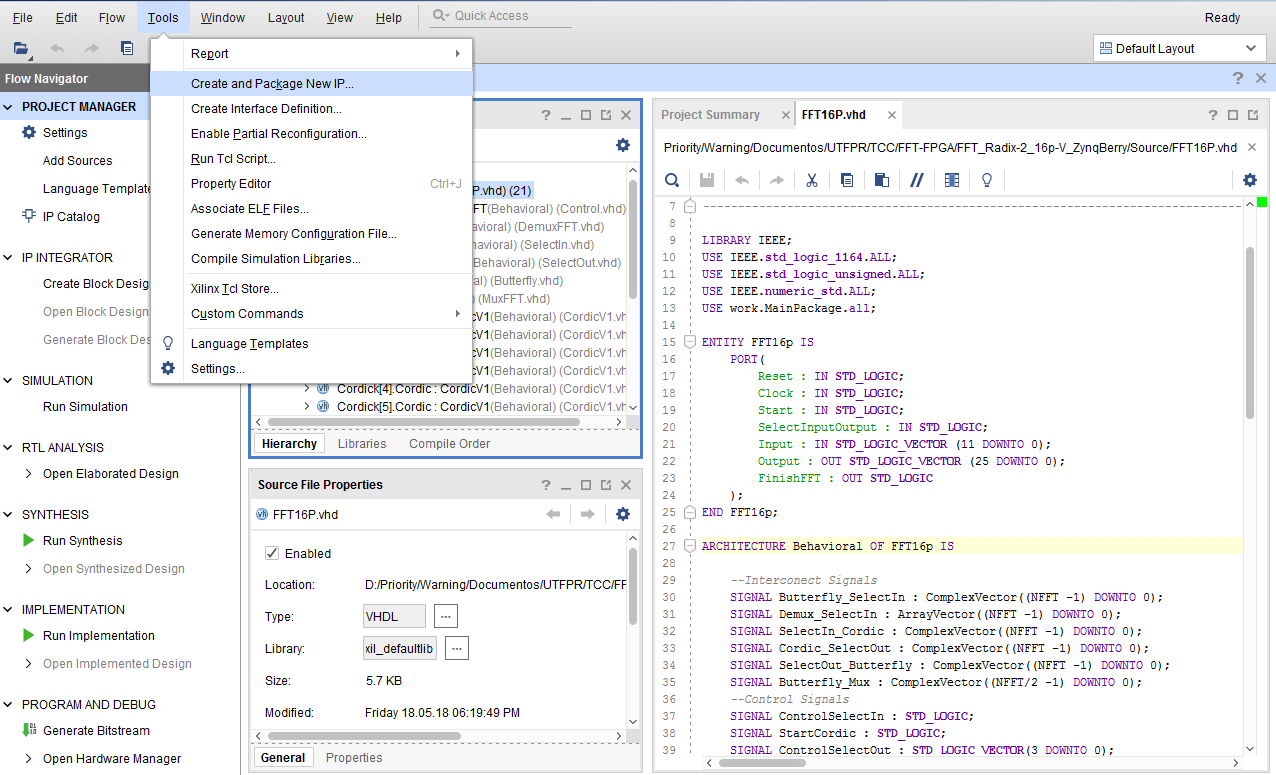
\includegraphics[width=0.8\linewidth]{Images/Anexo/CriacaoAXI.png}
	\caption{Caminho at� a ferramenta: \textit{Tools: Create and Package New IP}}
	\vspace{-3.5mm}
	\caption*{Fonte: Vivado HLx 2017.4}
	\label{fig:FerramentaIPA}
\end{figure}    
\vspace{5mm}

\vspace{5mm}
\begin{figure}[H]
	\centering
	\captionsetup{width=0.8\textwidth, font=footnotesize, textfont=bf}	
	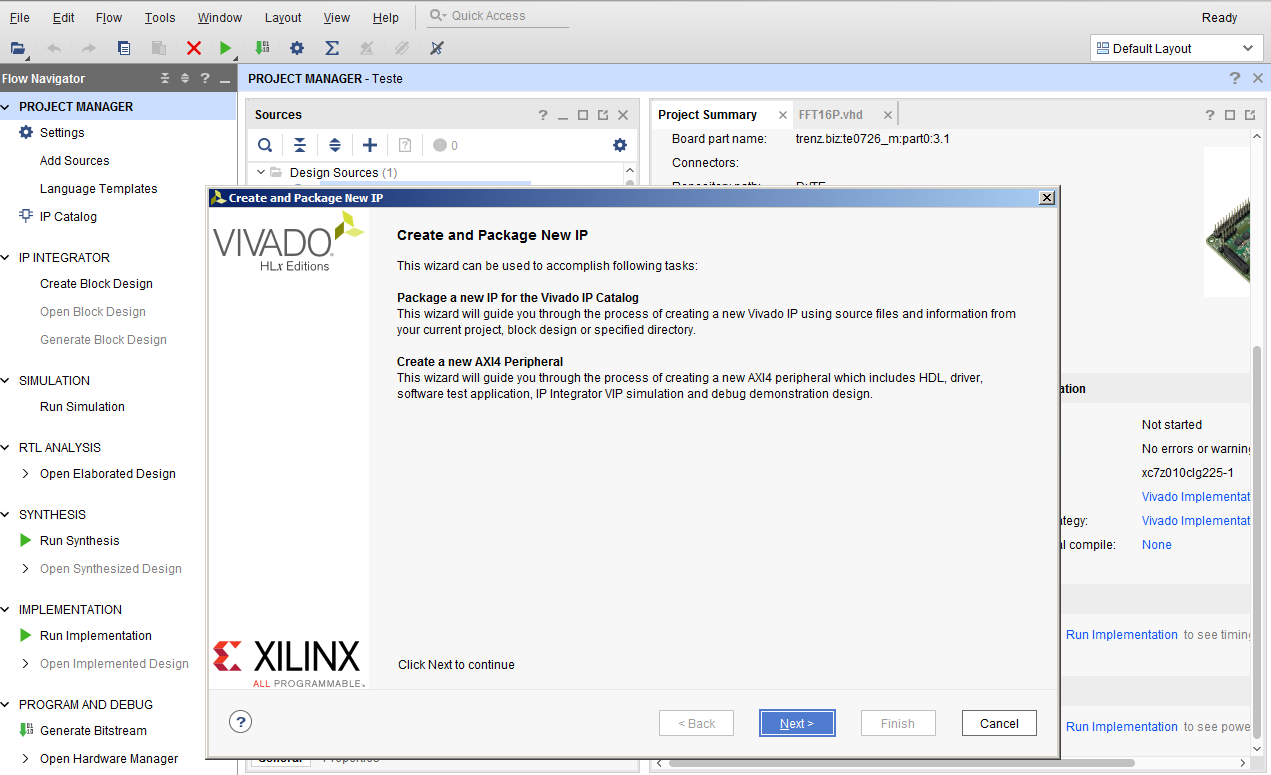
\includegraphics[width=0.8\linewidth]{Images/Anexo/CriacaoAXI2.png}
	\caption{Ferramenta de Cria��o e Empacotamento de Novas IPs}
	\vspace{-3.5mm}
	\caption*{Fonte: Vivado HLx 2017.4}
	\label{fig:FerramentaIPB}
\end{figure}    
\vspace{5mm}

\vspace{5mm}
\begin{figure}[H]
	\centering
	\captionsetup{width=0.8\textwidth, font=footnotesize, textfont=bf}	
	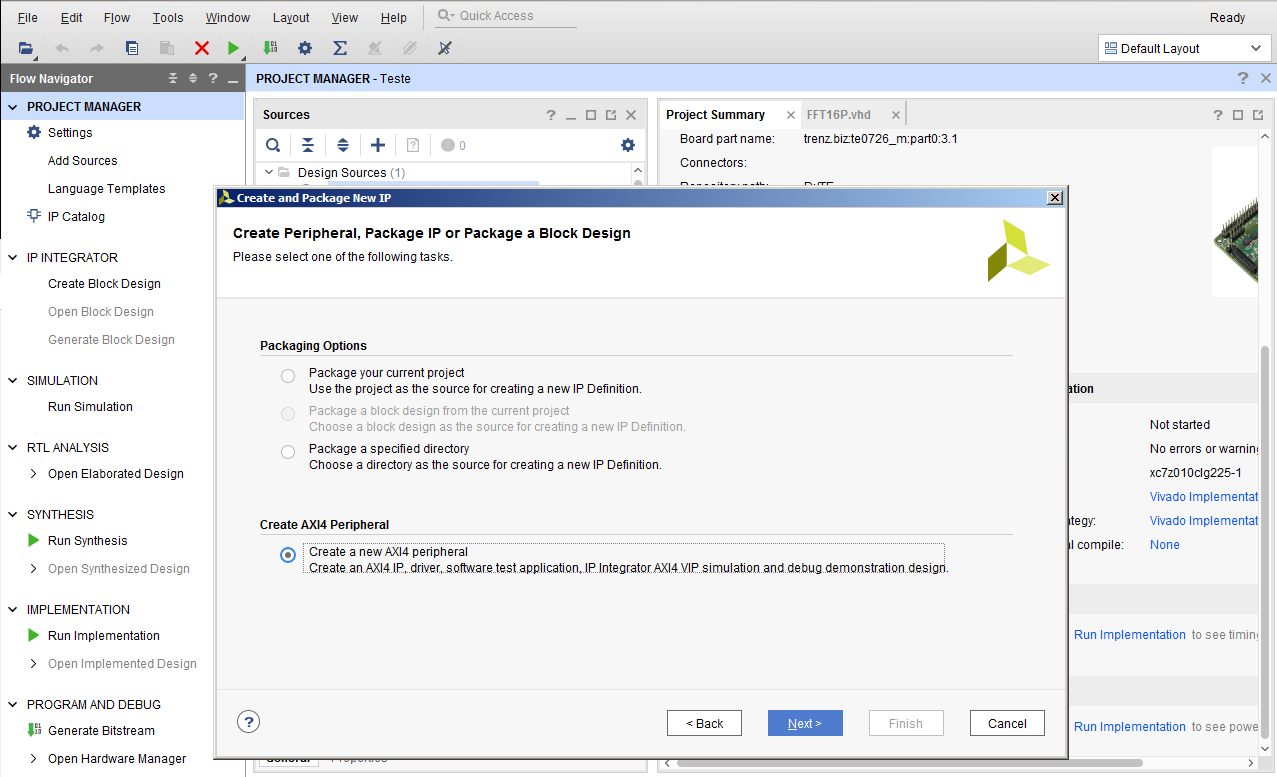
\includegraphics[width=0.8\linewidth]{Images/Anexo/CriacaoAXI3.png}
	\caption{Escolha da Op��o: \textit{Create a New Peripheral}}
	\vspace{-3.5mm}
	\caption*{Fonte: Vivado HLx 2017.4}
	\label{fig:FerramentaIPC}
\end{figure}    
\vspace{5mm}

\vspace{5mm}
\begin{figure}[H]
	\centering
	\captionsetup{width=0.8\textwidth, font=footnotesize, textfont=bf}	
	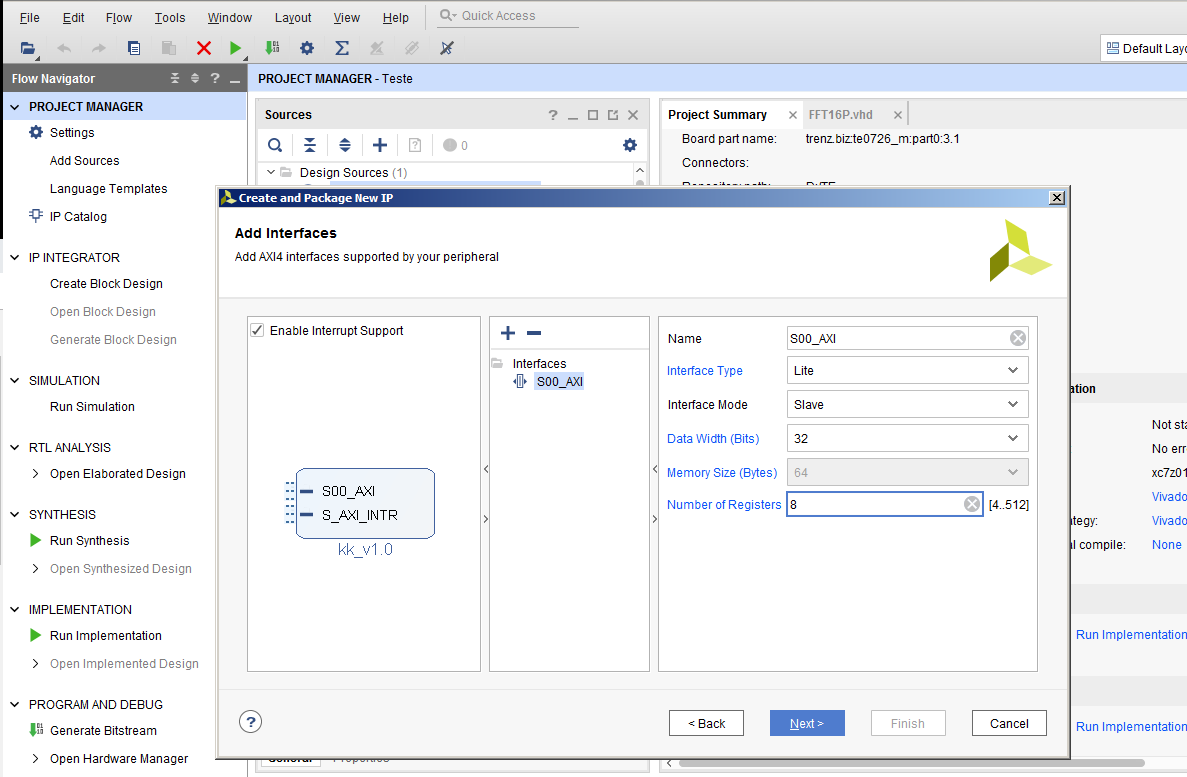
\includegraphics[width=0.8\linewidth]{Images/Anexo/CriacaoAXI4.png}
	\caption{Configura��es da nova IP}
	\vspace{-3.5mm}
	\caption*{Fonte: Vivado HLx 2017.4}
	\label{fig:FerramentaIPD}
\end{figure}    
\vspace{5mm}
 
Como pode ser observado na Figura (\ref{fig:FerramentaIPD}), para a cria��o da Interface AXI fora escolhido utilizar uma interface do tipo \textit{Lite}, no modo \textit{Slave}, com 8 endere�os de mem�ria, cada endere�o com 32 \textit{bits}, e ainda escolhida a op��o de habilita��o de interrup��es. Como � necess�rio transmitir apenas metade dos 16 pontos da FFT, ao fim do processo de c�lculo, s�o necess�rios 8 endere�os, sendo que cada endere�o de 32 \textit{bits} � divido de forma que, os 16 \textit{bits} mais significativos s�o destinados a parte real do sinal, e os 16 textit{bits} menos significativos para a parte imagin�ria. Para o envio dos dados, basta preencher cada um dos 8 endere�os de 32 \textit{bits}, com o valor de dois pontos de 16 \textit{bits} do sinal de entrada concatenados, considerando que os dados de entrada s�o puramente reais.

Ap�s a cria��o do Perif�rico AXI, foi necess�rio editar o c�digo Verilog do perif�rico, a fim de incluir o c�digo da implementa��o em VHDL da FFT de 16 pontos. Ap�s feitas tais altera��es, o design � salvo, e o Vivado geral os arquivos fonte para uma nova IP, que cont�m a implementa��o da FFT. Esta IP pode ser reutilizada em qualquer outra IDE de desenvolvimento de FPGAs, desde que  estas tenham suporte a AXI4.

	
\section{Programando o ZynqBerry}
	\label{cap:MapeantoProgZynq}
Para enviar os dados para a FFT em PL, � necess�rio que o processador Cortex-A9 consiga mapear o endere�o do perif�rico de Interface AXI relacionada com a FFT. Ap�s criar uma nova IP com a interface AXI, � necess�rio criar um novo Bloco de Design, no Vivado HLx 2017.4, como pode ser visto na Figura(\ref{fig:FFT16pImplementacaoA}).

\vspace{6mm}
\begin{figure}[H]
	\centering
	\captionsetup{width=1\textwidth, font=footnotesize, textfont=bf}	
	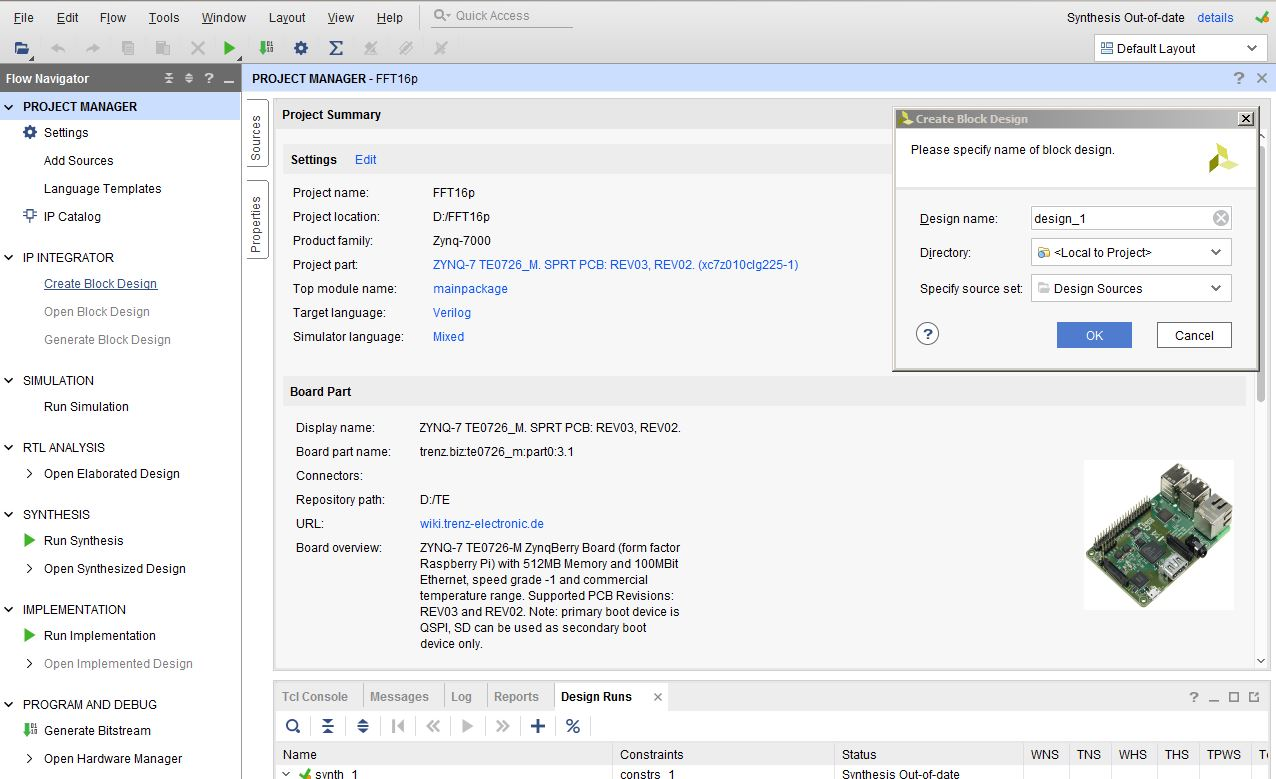
\includegraphics[width=1\linewidth]{Images/Apendice/FFT16pImplementacaoA.JPG}
	\caption{Cria��o de um Novo Bloco de Design}
	\vspace{-3.5mm}
	\caption*{Fonte: Vivado HLx 2017.4}
	\label{fig:FFT16pImplementacaoA}
\end{figure}
\vspace{6mm}

A partir deste novo bloco � preciso incluir uma IP \textit{ZYNQ7 Process System}, o qual representa o ambiente PS, juntamente com um IP AXI da FFT, criada no Anexo (\ref{cap:AXI}), e tamb�m uma unidade de controle de Interrup��es ($axi_int$).

\vspace{6mm}
\begin{figure}[H]
	\centering
	\captionsetup{width=1\textwidth, font=footnotesize, textfont=bf}	
	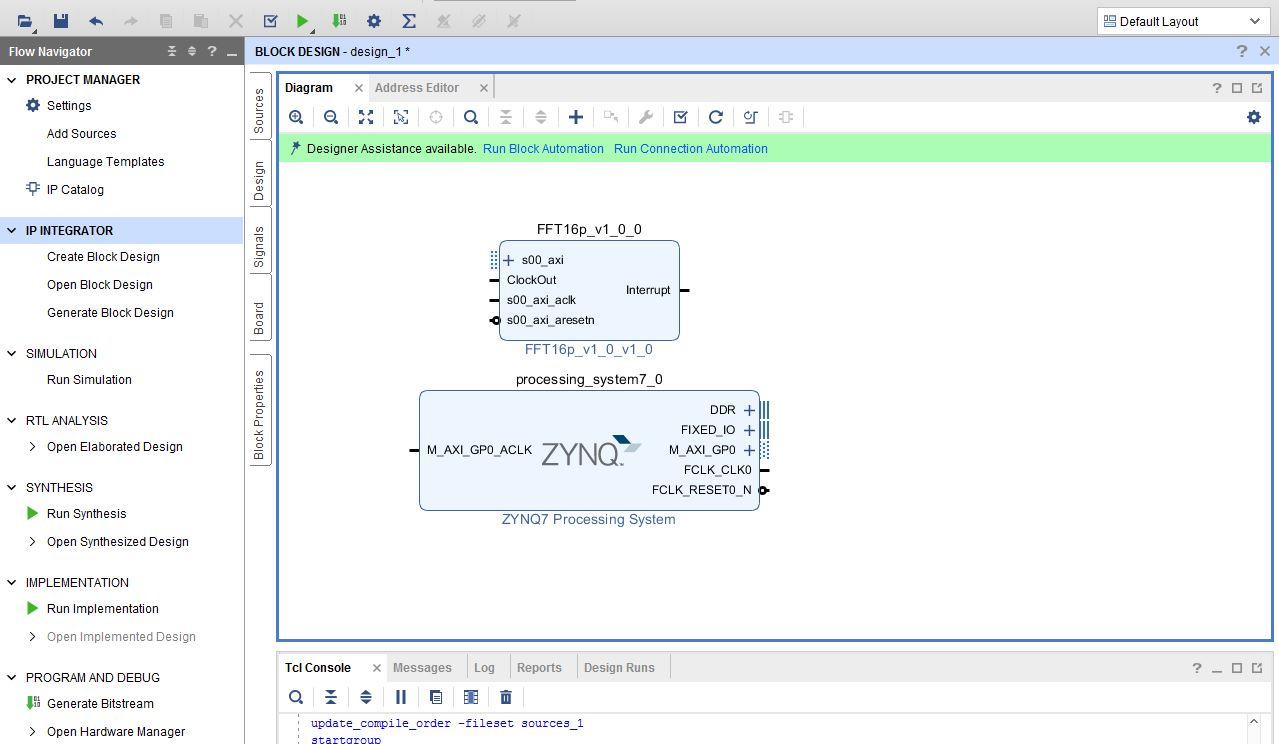
\includegraphics[width=1\linewidth]{Images/Apendice/FFT16pImplementacaoB.JPG}
	\caption{Cria��o de um Novo Bloco de Design}
	\vspace{-3.5mm}
	\caption*{Fonte: Vivado HLx 2017.4}
	\label{fig:FFT16pImplementacaoB}
\end{figure}
\vspace{6mm}

Ap�s a inclus�o deste 3 blocos � preciso realizar as devidas conex�es entre os blocos e a configura��o do bloco ZYNQ7. O Vivado 2017.4 disponibiliza ferramentas de automatiza��o das conex�es entre blocos e suas configura��es. Ap�s executar estas ferramentas, e conectar a sa�da da interrup��o do Bloco da FFT ao bloco de controle de interrup��es, o bloco de design � conclu�do, como mostra a Figura (\ref{fig:FFT16pImplementacaoC}).

\vspace{6mm}
\begin{figure}[H]
	\centering
	\captionsetup{width=1\textwidth, font=footnotesize, textfont=bf}	
	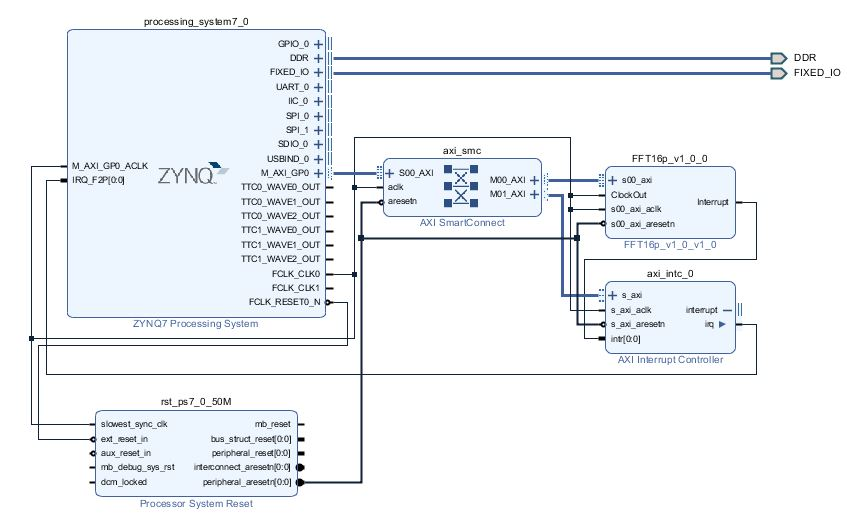
\includegraphics[width=1\linewidth]{Images/Apendice/FFT16pImplementacaoC.JPG}
	\caption{Bloco de Design para FFT 16 Pontos}
	\vspace{-3.5mm}
	\caption*{Fonte: Vivado HLx 2017.4}
	\label{fig:FFT16pImplementacaoC}
\end{figure}
\vspace{6mm}

Para identificar o endere�o de mem�ria que d� acesso aos registradores da Interface AXI do FFT, basta abrir a aba \textit{Adress Editor}. Como mostra a Figura (\ref{fig:FFT16pImplementacaoD}), o Vivado automaticamente reservou um endere�o de mem�ria que come�a em \textit{0x43C000000}. Logo, basta somente criar uma rotina em PS, para acessar este endere�o e enviar os dados.

\vspace{6mm}
\begin{figure}[H]
	\centering
	\captionsetup{width=1\textwidth, font=footnotesize, textfont=bf}	
	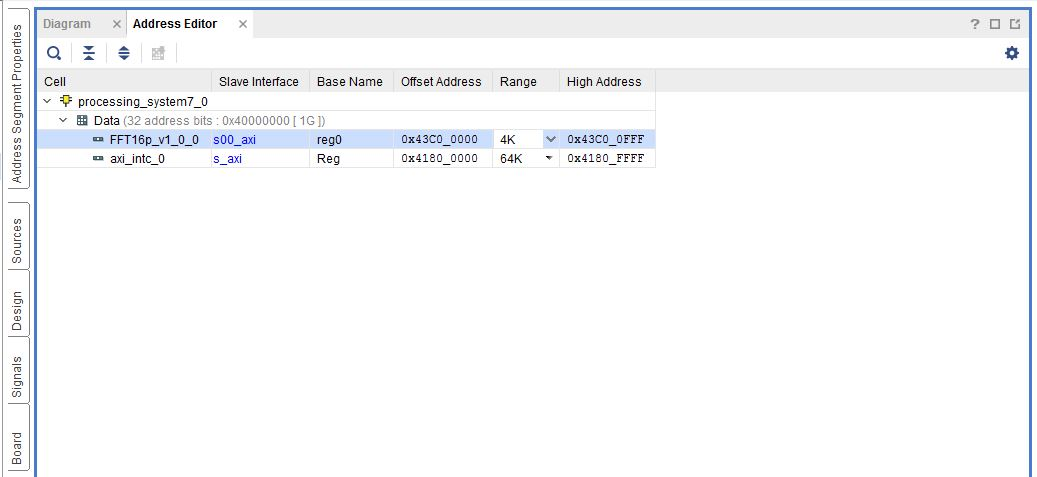
\includegraphics[width=1\linewidth]{Images/Apendice/FFT16pImplementacaoD.JPG}
	\caption{Endere�o de Mem�ria da Interface AXI FFT}
	\vspace{-3.5mm}
	\caption*{Fonte: Vivado HLx 2017.4}
	\label{fig:FFT16pImplementacaoD}
\end{figure}
\vspace{6mm}

Por fim, ap�s a inclus�o e configura��es de todos os blocos de IPs, basta rodar o comando \textit{Create HDL Wrapper}, para que o Vivado crie a hierarquia de c�digos HDL das IPs instanciadas. Em seguida � rodado a fun��o de s�ntese (\textit{Run Synthesis}), e implementa��o (\textit{Run Implementation}). Se todos os passos anteriores forem executados corretamente, ent�o o comando de gera��o do Bitstream (\textit{Generate Bitstream}) pode ser executado.

Para programar a parte PS e tamb�m carregar a FPGA com o arquivo \textit{Bitstream} gerado, o projeto de \textit{hardware} feito no Vivado HLx precisa ser exportado para um projeto de \textit{hardware/software} e ent�o carregado para dentro do IDE Vivado SDK 2017.4. Para isso, basta escolher a op��o  File, na barra de tarefas do projeto aberto no Vivado HLx, ir em \textit{Export}, em seguida em \textit{Export Hardware}. Ao fim, basta abrir o Vivado SDK, pela op��es \textit{Launch SDK}.

Ap�s exportar o projeto para o Vivado SDK, o PS fora programado para utilizar a interface UART0 do ZynqBerry para receber e enviar os dados retirados do endere�o de mem�ria da interface AXI da FFT de 16 pontos implementada. Para realizar esta opera��o foram necess�rios apenas algumas opera��es com ponteiros de mem�ria. Ao fim, basta executar a compila��o e \textit{debugger} do Vivado SDK, para ent�o realizar os testes de funcionamento da FFT. 
	
\section{Implementando a FFT 1024 Pontos}
	Implementar uma FFT de 1024 pontos � importante para comprovar a efici�ncia da arquitetura implementada, j� que � mais comum encontrar na literatura FFT de 1024 pontos. Portanto, reutilizando os  m�dulos CORDIC usados na FFT de 16 pontos, � desenvolvido uma nova arquitetura para a FFT de 1024 pontos. 

A arquitetura implementada para a FFT de 16 pontos possui um processamento paralelo em rela��o aos m�dulos de c�lculo CORDIC, de modo que todas as opera��es de rota��o de vetores, para um determinado n�vel, s�o realizadas paralelamente. Para a implementa��o de uma FFT com 1024, ou mesmo 512 pontos, n�o seria poss�vel utilizar a mesma arquitetura paralela em rela��o as unidades CORDIC. Pois o n�mero de conex�es, \textit{mux} e \textit{Flip-flops} presentes na FPGA n�o seriam suficientes para tal tarefa.

\vspace{5mm}
\begin{figure}[H]
	\centering
	\captionsetup{width=\textwidth, font=footnotesize, textfont=bf}	
	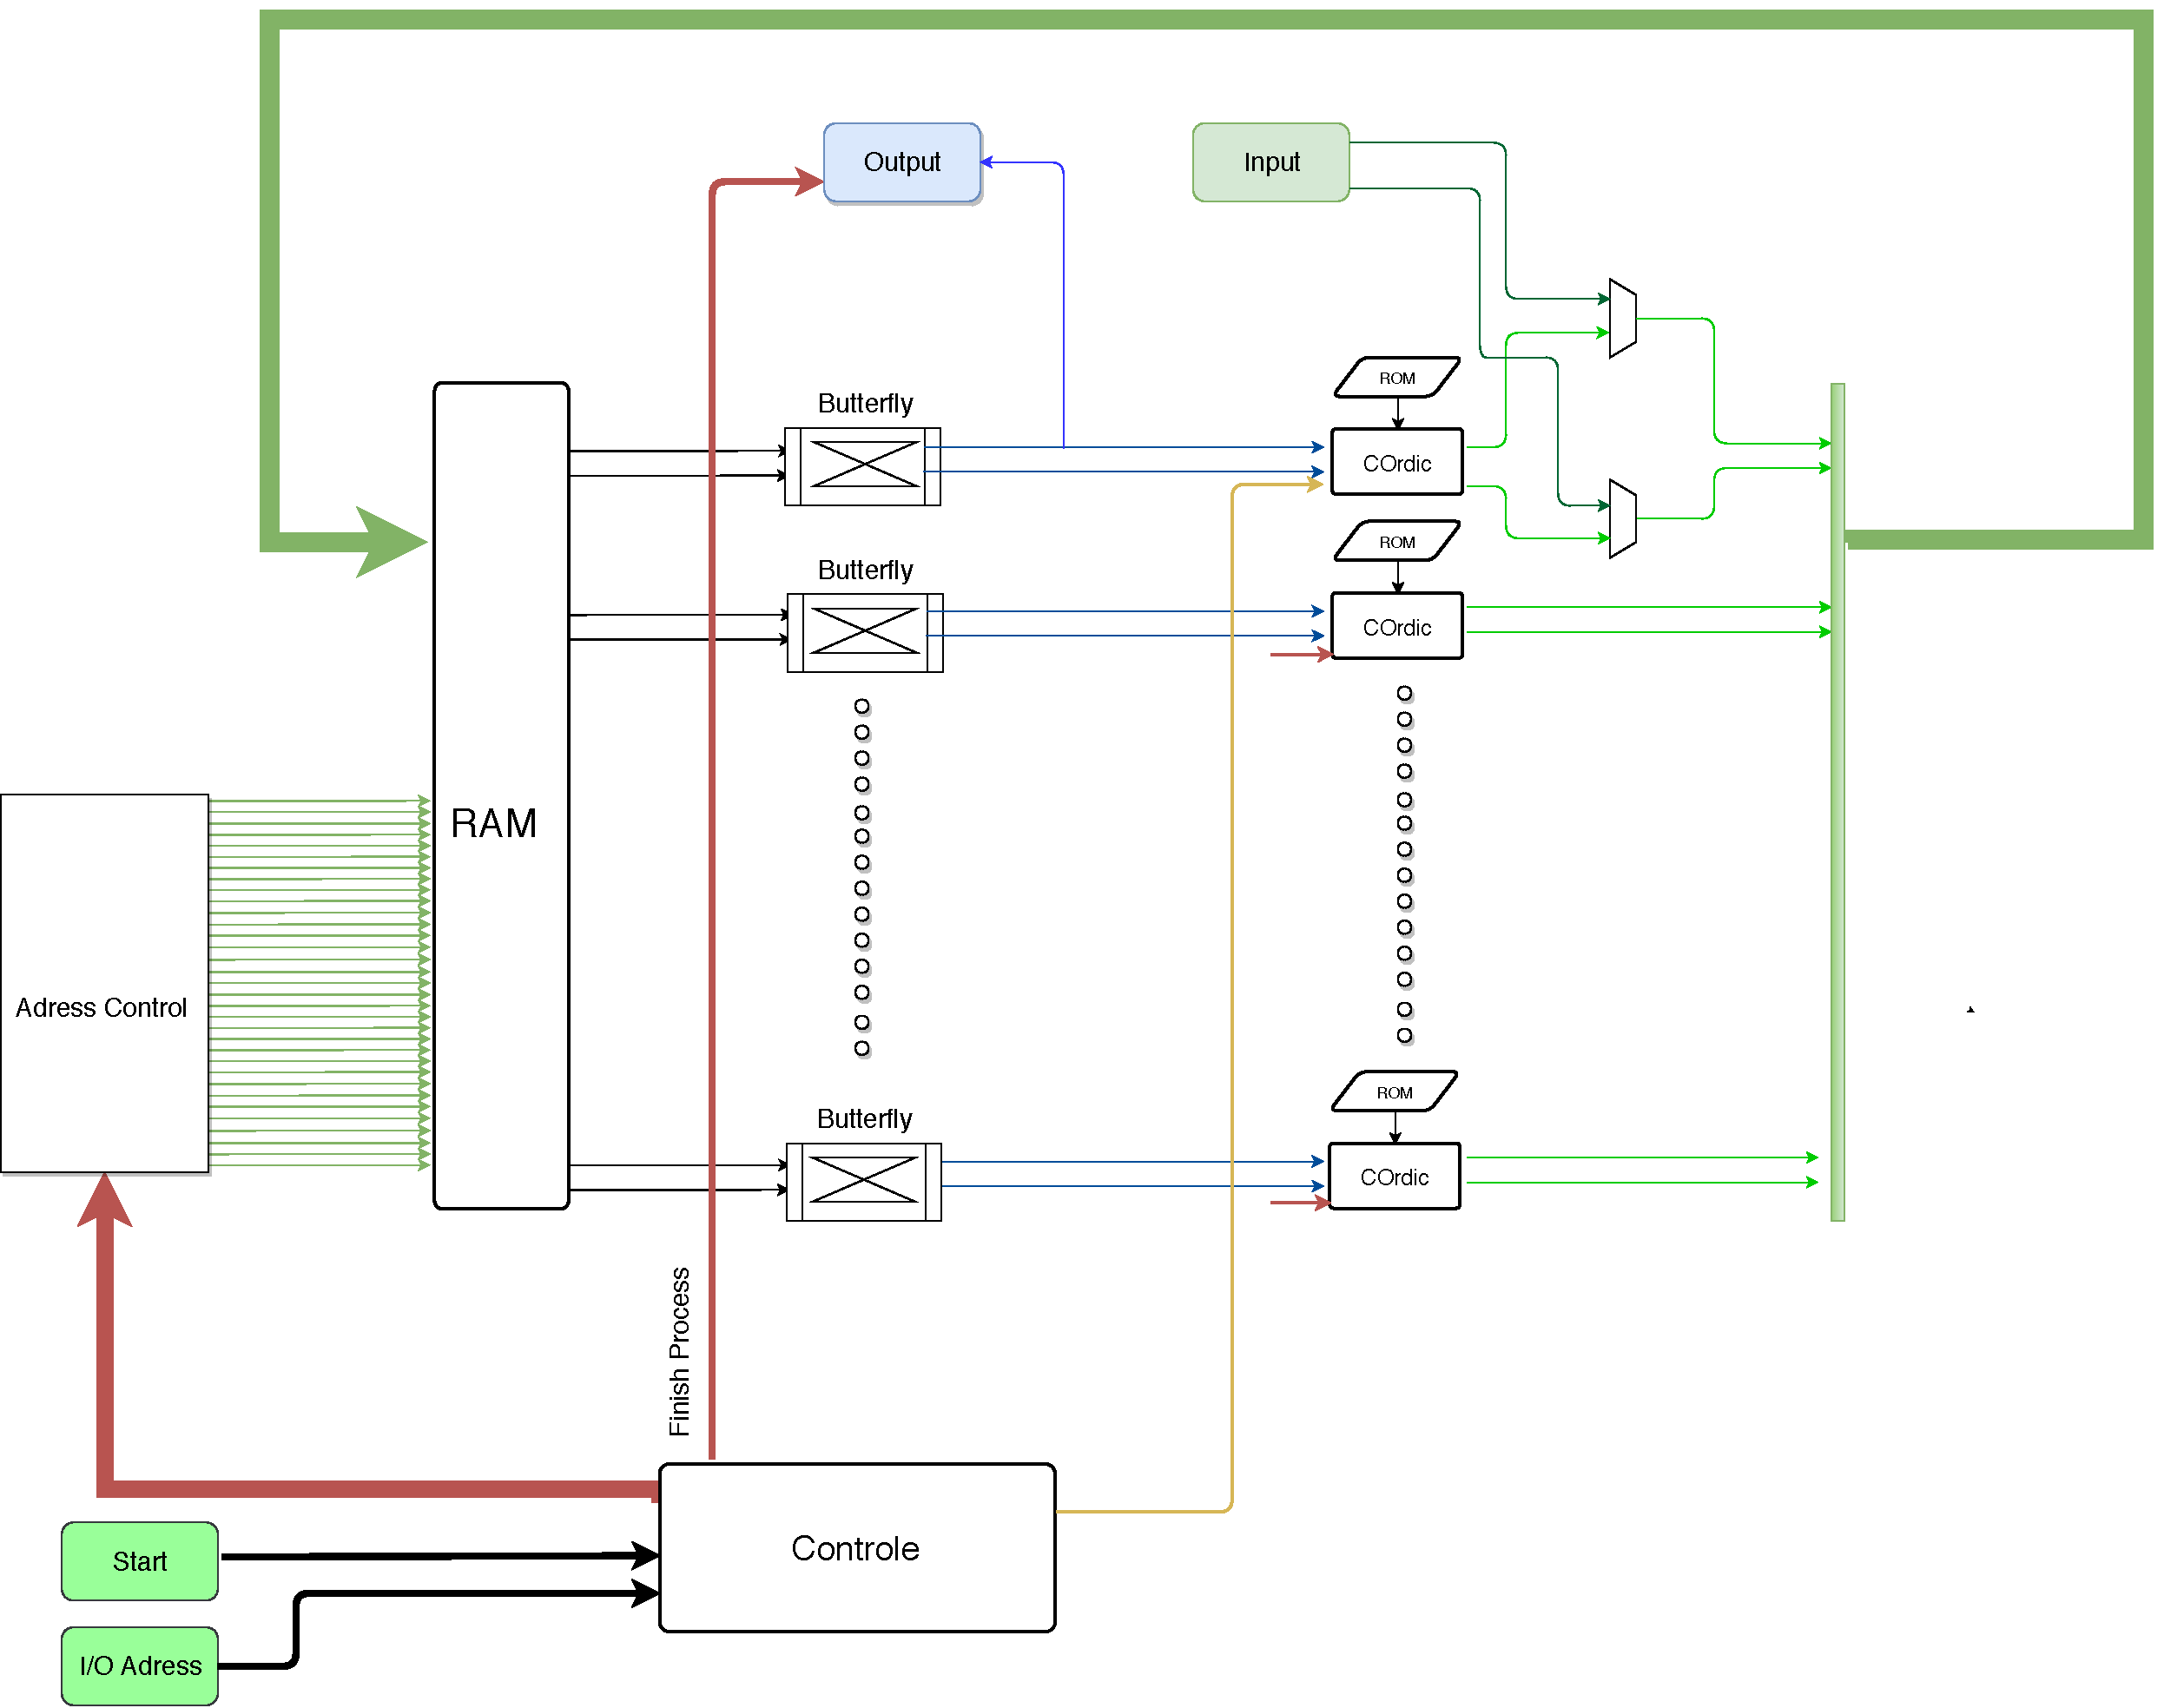
\includegraphics[width=\linewidth]{Images/MateriaisMetodos/ArquiteturaFFT1024.pdf}
	\caption{Arquitetura FFT 1024 Pontos Implementada}
	\vspace{-3.5mm}
	\caption*{Fonte: Autoria Pr�pria}
	\label{fig:ArchitectureFFT1024p}
\end{figure}    
\vspace{5mm}

A solu��o adotada para montar a FFT de 1024 pontos, foi realizar as opera��es CORDIC de cada n�vel da FFT de modo fracion�rio. Uma FFT de 1024 pontos possu� ao total 10 n�veis de c�lculo ($log_2 N$), e 512 opera��es CORDIC por n�vel. Se for utilizado 8 unidades CORDIC em paralelo, para calcular conjuntos de 8 opera��es por itera��o, � poss�vel realizar o calculo de um n�vel reutilizando as unidades CORDIC 64 vezes.  Por�m para esta tarefa � necess�rio utilizar um bloco RAM, para armazenar os 1024 pontos, e permitir o acesso a 16 pontos a cada itera��o. A Figura (\ref{fig:ArchitectureFFT1024p}) apresenta um diagrama da arquitetura implementada para a FFT de 1024 pontos.

A FFT de 16 pontos n�o possui nenhum bloco de memoria RAM (\textit{BRAM}), utilizando apenas registradores para operar as itera��es, o que a torna menos exigente em termos de recursos da FPGA. J� uma FFT de 1024 requer n�o apenas uma bloco comum de RAM, mas uma mem�ria de acesso m�ltiplo, j� que se faz necess�rio ler e escrever em 16 pontos diferentes a cada itera��o. Pois, caso contr�rio, seria necess�rio transferir cada ponto da FFT individualmente para cada unidade CORDIC em paralelo, reduzindo assim o desempenho da FFT. Para criar algo como um bloco de RAM com 16 canais, foram criados 16 blocos de mem�ria RAM \textit{single port}, cada um com 64 endere�os de mem�ria. A entrada e sa�da de dados destes blocos � ligado a uma rede de multiplexadores, os quais ordenam os dados a serem armazenados em blocos espec�ficos. 

No diagrama da Figura (\ref{fig:ArchitectureFFT1024p}), a FFT de 1024 pontos al�m de dispor de uma unidade \textit{RAM} de m�ltiplos acessos, ainda contem um bloco \textit{Adress Control}, o qual � respons�vel por endere�ar os resultados das opera��es CORDIC para o espa�o de mem�ria adequado no bloco \textit{RAM}. 

A entrada de dados nesta arquitetura � feita por meio do bloco \textit{Input}. Este bloco separa os dados seriais de reais de 32 \textit{bits} oriundos de PS, em dois sinais reais de 16 \textit{bits}, e por meio de dois multiplexadores, insere esses dados nas duas primeiras portas de dados do bloco \textit{RAM}. Enquanto a interface AXI estiver repassando ao m�dulo da FFT os dados de entrada, e endere�ando estes por meio da porta \textit{I/O Adress}, o bloco de \textit{Controle} vai preenchendo a mem�ria \textit{RAM} com os dados de entrada. 

Ap�s preencher todos os dados da \textit{RAM}, a interface AXI, dispara a porta \text{start}, e a opera��o da FFT � iniciada. Ao final, o bloco de \textit{Controle} aciona a porta \textit{Finish Process}, provocando uma interrup��o em PS, notificando sobre o fim da opera��o. Ent�o os dados s�o transferidos ao PS, de acordo com o endere�o requisitado pela interface AXI na porta \textit{I/O Adress}, repassando os dados pela primeira porta de leitura do bloco \textit{RAM}.
  

